\documentclass{article}
\usepackage{graphicx}
\usepackage{amsmath}
\usepackage{enumitem}
\usepackage{float}
\usepackage{listings}
\usepackage{xcolor}
\usepackage{caption}
\usepackage[a4paper, margin=1in]{geometry}

% Custom information
\newcommand{\className}{Course: Automatic Control Systems – ASEN 5114-001 – Spring 2025}
\newcommand{\professorName}{Professor: Dale Lawrence}
\newcommand{\taName}{Teaching Assistant: Anantha Dhruva}
\title{Project 2 \\ \className \\ \professorName \\ \taName}
\author{Steve Gillet}
\date{\today}

\lstdefinestyle{matlabstyle}{
    language=Matlab,              % Specify the language
    basicstyle=\ttfamily\footnotesize\color{black}, % Code font
    keywordstyle=\color{blue}\bfseries, % Keywords in blue
    stringstyle=\color{orange},    % Strings in orange
    commentstyle=\color{magenta}, % Comments in magenta
    numbers=left,                 % Line numbers on the left
    numberstyle=\tiny\color{black},% Line number style
    stepnumber=1,                 % Line number increment
    breaklines=true,              % Line breaking
    frame=single,                 % Border around code
    backgroundcolor=\color{white},
    tabsize=4,                    % Tab size
    showstringspaces=false,       % Don't show spaces in strings
}

\renewcommand{\thesection}{\arabic{section})}
\renewcommand{\thesubsection}{\arabic{section}.\alph{subsection})}

\begin{document}

\maketitle

\textit{This project will build on Project 1, applying state space modeling and design methods to control the attitude of a spacecraft mockup model. A state space model for the spacecraft will be obtained by fitting the empirical frequency response model. A controller will be designed using state variable feedback and state observation methods, then implemented in a closed loop simulation. Here however, the controller will be in state-space form, rather than the transfer function form from Project 1.} \\
\textit{The project will be carried out using the same teams as for Project 1, and a single report will be submitted by each team. The report should include an introduction, sections for each of the following parts, and a conclusion pointing out key lessons learned or difficulties. All team members should contribute approximately equally to the conduct of the project and the write-up, and a short description of member contributions is required. The report is due at 11:59 pm on Monday May 5.}

\section{}
\textit{[20 pts] Use the empirical frequency response data taken during Project 1 to fit an analytical transfer function model relating input reaction wheel torque (in $\mathrm{mN}-\mathrm{m}$) to output body angular deflection (in rad). Overplot the empirical and analytic model frequency responses in Bode plot format. Try to match the damping in the empirical data, and modify the dynamics to capture the phase at low frequencies seen in the empirical data. Treat the dynamics around $3 \mathrm{~Hz}$ and above as unmodeled. Using this analytic transfer function model to create a minimal state space representation of the system.}

I used the same technique and code that I used in the previous project, basically capturing the dynamics using second-order polynomials of the form \((s^2 + 2\zeta\omega_n s + \omega_n^2)\) to capture the resonances and antiresonances and a couple of extra poles to capture the magnitude and phase drop-off.

Here is the code:

\begin{lstlisting}[style=matlabstyle]
dataTable = readtable('data.xlsx', 'VariableNamingRule', 'preserve');
data = table2array(dataTable);

[uniqueFreq, ia] = unique(data(:,1));
n = size(uniqueFreq,1);
pResponse = zeros(n,3);

for i = 1:n
    idx = ia(i);
    pResponse(i,1) = 20*log10(data(idx,2)) - 20*log10(data(i,1));
    pResponse(i,2) = data(idx,3)*180/pi - 90;
    pResponse(i,3) = data(idx,1)*2*pi;
end

K = 1;
zetaZ = 0.05;
zetaP = 0.1;
omegaZ = 4.60118;
omegaP = 8.34686;

num = K*[1 zetaZ*omegaZ omegaZ^2];
den = [1 zetaP*omegaP omegaP^2 0];
pole = [1 0.65];
den = conv(den, pole);
estTF = tf(num,den);

% Generate Bode plot data for the transfer function
[mag, phase, w] = bode(estTF);
mag = squeeze(mag); % Convert to 1D array
phase = squeeze(phase); % Convert to 1D array

% Plot empirical data and transfer function Bode plot on the same figure
clf; figure(1); 

% Magnitude plot
subplot(2,1,1);
semilogx(pResponse(:,3), pResponse(:,1), 'b', 'LineWidth', 1.5); % Empirical data in blue
hold on;
semilogx(w, 20*log10(mag), 'r--', 'LineWidth', 1.5); % Transfer function in red dashed
grid on;
ylabel('Magnitude (dB)');
title('Comparison of Empirical Data and Transfer Function Bode Plot');
legend('Empirical Data', 'Transfer Function');
xlim([0.5, 50]);

% Phase plot
subplot(2,1,2);
semilogx(pResponse(:,3), pResponse(:,2), 'b', 'LineWidth', 1.5); % Empirical data in blue
hold on;
semilogx(w, phase, 'r--', 'LineWidth', 1.5); % Transfer function in red dashed
grid on;
xlabel('Frequency (rad/s)');
ylabel('Phase (deg)');
legend('Empirical Data', 'Transfer Function');
xlim([0.5, 50]);    
\end{lstlisting}

Here is the output:

\begin{figure}[H]
\centering
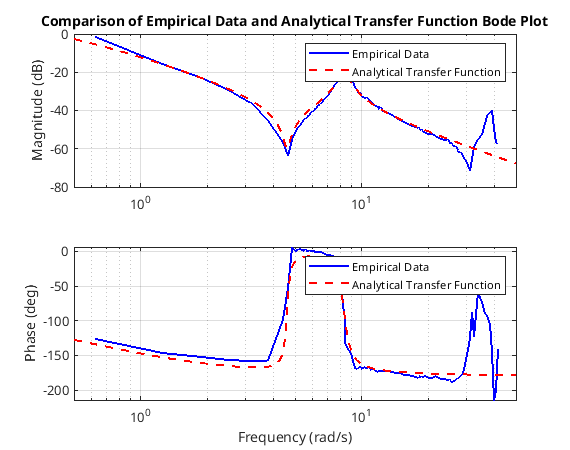
\includegraphics[width=0.8\textwidth]{anVemp.png}
\label{fig:anVemp}
\end{figure}

I then used the 'ss2tf' Matlab function to get the state space realization from the transfer function I had developed.

The resulting state space matrices look like this:

\begin{itemize}
    \item \textbf{A matrix}:
    \[
    A = \begin{bmatrix}
        -1.4847 & -70.2126 & -45.2855 & 0 \\
        1.0000 & 0 & 0 & 0 \\
        0 & 1.0000 & 0 & 0 \\
        0 & 0 & 1.0000 & 0
    \end{bmatrix}
    \]
    
    \item \textbf{B matrix}:
    \[
    B = \begin{bmatrix}
        1 \\
        0 \\
        0 \\
        0
    \end{bmatrix}
    \]
    
    \item \textbf{C matrix}:
    \[
    C = \begin{bmatrix}
        0 & 1.0000 & 0.2301 & 21.1709
    \end{bmatrix}
    \]
    
    \item \textbf{D matrix}:
    \[
    D = \begin{bmatrix}
        0
    \end{bmatrix}
    \]
\end{itemize}

\section{}
\textit{[20 pts] Determine suitable closed loop pole locations so that the closed loop tracking bandwidth ($-3 \mathrm{~dB}$) is at least $1 \mathrm{~Hz}$. Design a state variable feedback controller to place closed loop poles in these locations. Plot the closed loop tracking frequency response (rad/rad), and the closed loop frequency response from reference input to plant input ( $\mathrm{mN}-\mathrm{m} / \mathrm{rad}$ ). Plot the (negative) loop gain of this control system using the analytic plant model in both a Bode and Nyquist format. Comment on the stability margins of this design relative to those obtained in project 1.}

I got the initial open loop poles using the 'eig' function on the A matrix:

\[
\begin{bmatrix}
0.0000 + 0.0000i \\
-0.4173 + 8.3364i \\
-0.4173 - 8.3364i \\
-0.6500 + 0.0000i
\end{bmatrix}
\]

I then decided to use a similar strategy as in the first project to create some pole/zero cancellation to reduce the effects of the resonances, however this time I wanted to only partially cancel them to make sure I wouldn't create instability anywhere else so I placed the dominant poles at $-0.615 \pm 4.5997$, just to the left of the analytical transfer function zeros.
Then I placed the other two poles at -10 and -12 so that they decayed quickly.
I then calculated the K matrix using 'place' and the F matrix using $F = \left[ C (A + B K)^{-1} B \right]^{-1}$ to get good tracking.

\begin{lstlisting}[style=matlabstyle]
[A,B,C,D] = tf2ss(num, den);

disp(eig(A));

desiredPoles = [-0.615 + 4.5997i, -0.615 - 4.5997i, -10, -12];
K = place(A, B, desiredPoles);
F = inv(C*inv(-A+B*K)*B);

sysCL = ss(A-B*K, B*F, C, D);
figure(2);
bode(sysCL);
title('Close Loop Tracking Frequency Response');
grid on;    
\end{lstlisting}

Then I plotted the closed loop frequency response:

\begin{figure}[H]
\centering
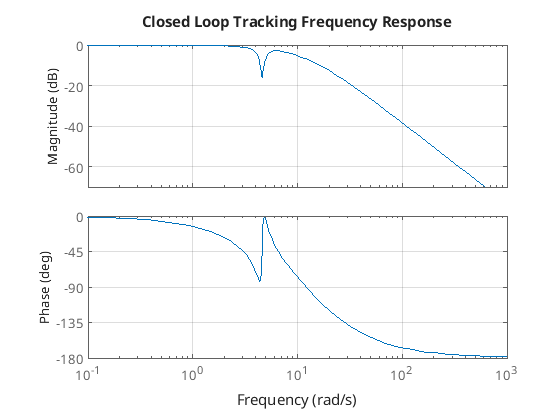
\includegraphics[width=0.8\textwidth]{clFreqResp.png}
\label{fig:clFreqResp}
\end{figure}

The closed loop frequency response from reference input to plant input:

\begin{figure}[H]
\centering
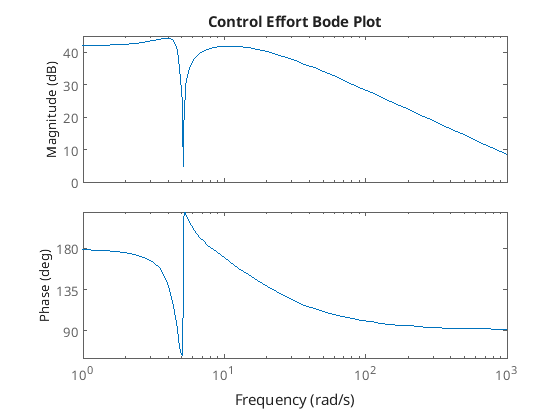
\includegraphics[width=0.8\textwidth]{r2pFreqResp.png}
\label{fig:r2pFreqResp}
\end{figure}

The (negative) loop gain Bode and Nyquist plots:

\begin{figure}[H]
\centering
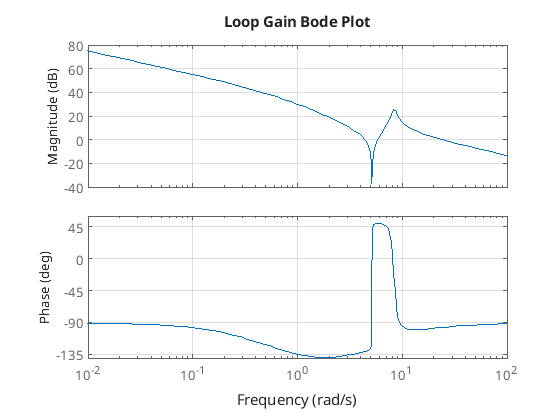
\includegraphics[width=0.8\textwidth]{loopGainFreqResp.png}
\label{fig:loopGainFreqResp}
\end{figure}

\begin{figure}[H]
\centering
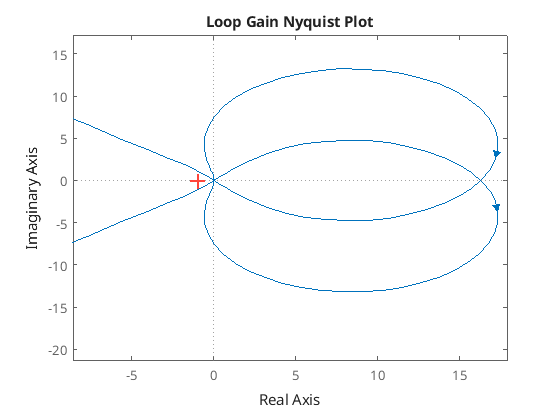
\includegraphics[width=0.8\textwidth]{loopGainNyquist.png}
\label{fig:loopGainNyquist}
\end{figure}

So the stability margin here is not as good as it was in the previous project, here the phase margin is 49 and the gain margin is infinite for the loop gain.
In the previous proect the phase margin was 108 degrees with infinite gain margin but in that case I had used a compensator to completely cancel the resonances so while the closed loop behavior would have been better, there would be instabilities elsewhere.

\section{}
\textit{[20 pts] Simulate the state variable feedback controller design in part 2 including a saturation at the plant input corresponding to $+/-67 \mathrm{mN} \cdot \mathrm{m}$ limits on the reaction wheel motor actuator. Use sinusoidal reference inputs of 0.1 and $1.0 \mathrm{~Hz}$, at amplitudes small enough to avoid actuator saturation. Also use a step input of height 0.1 rad. Show plant output and plant input responses. Compare them with the frequency responses from part 2.}

I created the simulation using the Simulink extension of Matlab, I built the system using gains and integrators as you can see in the block diagram below:

\begin{figure}[H]
\centering
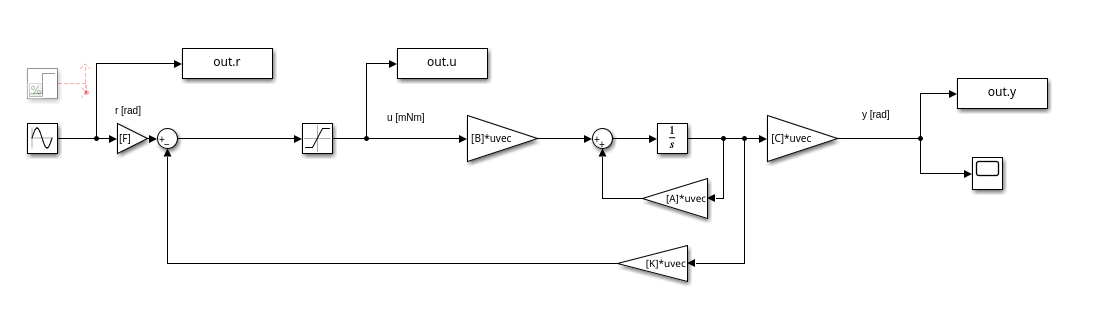
\includegraphics[width=0.8\textwidth]{simBlock.png}
\label{fig:simBlock}
\end{figure}

Then I simulated a step reference input of 0.1 rad and a sine reference input of 0.1 rad at 0.1 and 1 Hz and plotted the results:

\begin{figure}[H]
\centering
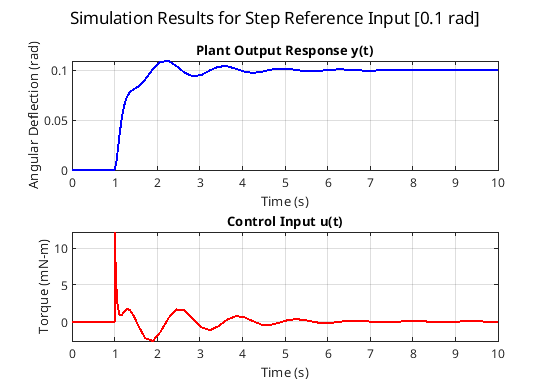
\includegraphics[width=0.8\textwidth]{stepResp.png}
\label{fig:stepResp}
\end{figure}

\begin{figure}[H]
\centering
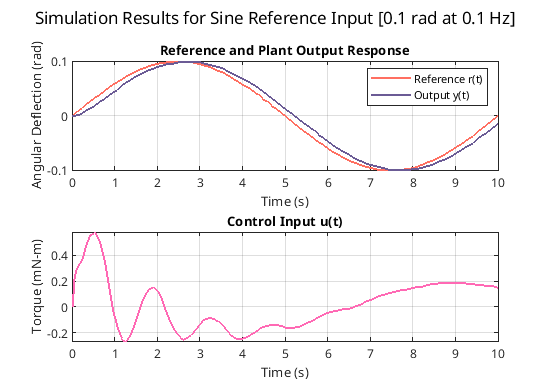
\includegraphics[width=0.8\textwidth]{sinRespPointOne.png}
\label{fig:sinRespPointOne}
\end{figure}

\begin{figure}[H]
\centering
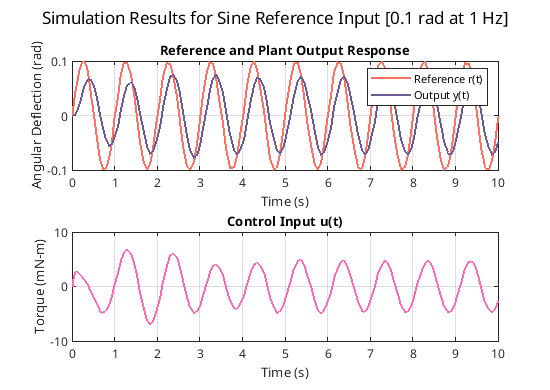
\includegraphics[width=0.8\textwidth]{sinRespOne.png}
\label{fig:sinRespOne}
\end{figure}

You can see that the tracking is pretty close at 0.1 Hz and matches up with the 70\% amplitude and 45 degree phase lag at 1 Hz that we would expect from the closed loop frequency response calculated earlier.

\section{}
\textit{[20 pts] Design a full state observer so that state observation errors have settling times (5 percent) of $3 \mathrm{~sec}$. or less. Plot the (negative) loop gain (loop cut at plant input) for the combined observer/state estimate feedback controller, in both Bode and Nyquist formats, using both the analytic and empirical model for the plant. Comment on the stability margins of your combined observer/state feedback controller design. Redesign the observer, if necessary, to retain 40 degrees of phase margin and $10 \mathrm{~dB}$ of gain margin.}

In order to design the observer, I just started by multiplying the closed loop poles by 5 as a rule of thumb and then calculated the settling time using the $t_s = \frac{3}{a}$ approximation and got about 1 second for the dominant poles which fits the requirements.
Then I used the 'place' function to get the observer gain matrix L and created and plotted the results using the following code:

\begin{lstlisting}[style=matlabstyle]
scalingFactor = 5;
desiredObserverPoles = [scalingFactor*-0.615 + 4.5997i, scalingFactor*-0.615 - 4.5997i, scalingFactor*-10, scalingFactor*-12];

disp(desiredObserverPoles);

L = place(A', C', desiredObserverPoles)';

obsSys = ss(A-B*K-L*C, L, -K, 0);
analG = ss(A, B, C, D);

obsLGsys = -obsSys*analG;
figure(9);
margin(obsLGsys);
title('Analytical Observer Loop Gain Bode Plot');
grid on;
xlim([0.5, 50]);

figure(10);
nyquist(obsLGsys);
title('Analytical Observer Loop Gain Nyquist Plot');

empG = frd(10.^(pResponse(:,1)/20) .* exp(1j * deg2rad(pResponse(:,2))), pResponse(:,3));

empObsLGsys = -obsSys*empG;
figure(11);
margin(empObsLGsys);
title('Empirical Observer Loop Gain Bode Plot');
grid on;
xlim([0.5, 50]);

figure(12);
nyquist(empObsLGsys);
title('Empirical Observer Loop Gain Nyquist Plot');
\end{lstlisting}    

The results are below:
\begin{figure}[H]
\centering
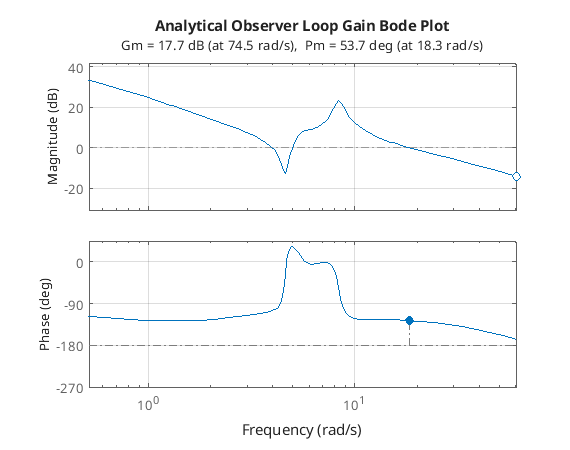
\includegraphics[width=0.8\textwidth]{analObsResp.png}
\label{fig:analObsResp}
\end{figure}

\begin{figure}[H]
\centering
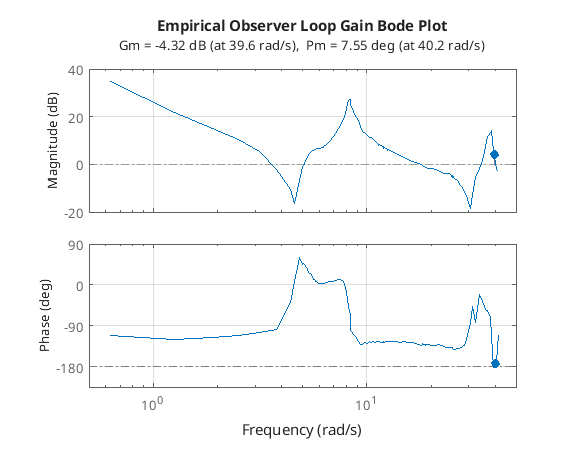
\includegraphics[width=0.8\textwidth]{empObsResp.png}
\label{fig:empObsResp}
\end{figure}

You can see the analytical and empirical observer systems both line up pretty well and the phase and gain margin meet the requirements.

\section{}
\textit{[20 pts] Simulate the combined observer/state feedback control system, using the same reference inputs as in part 3. Comment on the effects of adding an observer in your state feedback control design.}

I started by creating the observer system in Simulink, using the system before but adding an observer path and connecting K to $\hat{x}$ instead of $x$.

\begin{figure}[H]
\centering
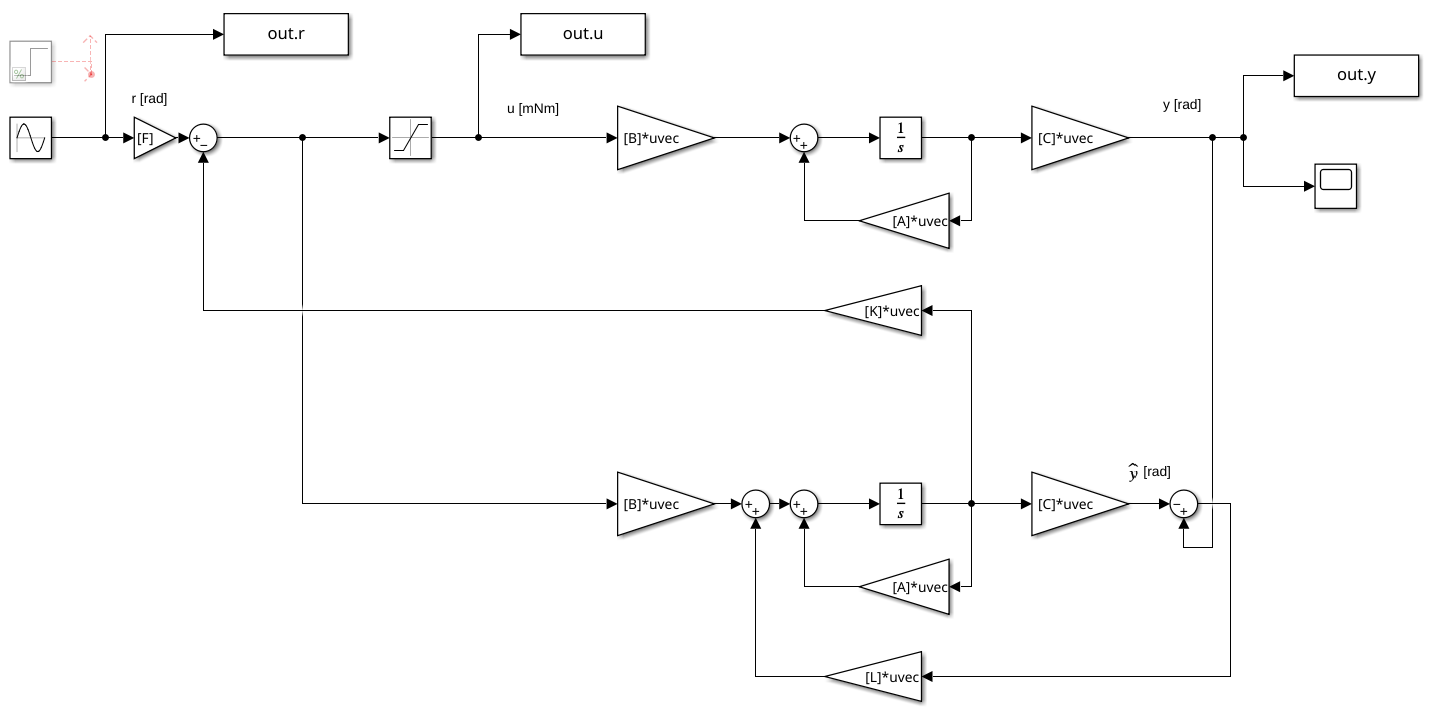
\includegraphics[width=\textwidth]{obsBlockDiagram.png}
\label{fig:obsBlockDiagram}
\end{figure}

The I simulated and plotted the response to the sine and step inputs.

\begin{figure}[H]
\centering
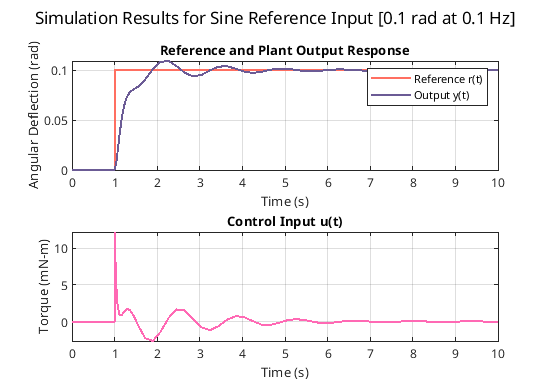
\includegraphics[width=0.8\textwidth]{obsStepResp.png}
\label{fig:obsStepResp}
\end{figure}

\begin{figure}[H]   
\centering
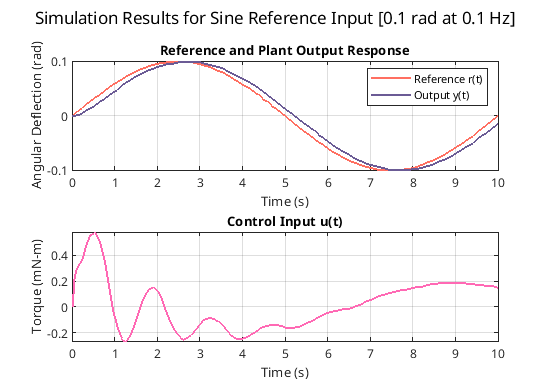
\includegraphics[width=0.8\textwidth]{obsSinRespPointOne.png}
\label{fig:obsSinRespPointOne}
\end{figure}

\begin{figure}[H]
\centering
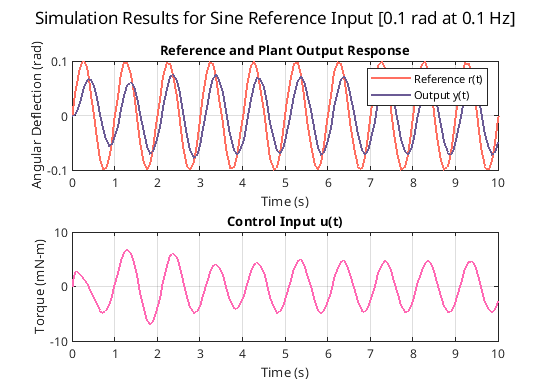
\includegraphics[width=0.8\textwidth]{obsSinRespOne.png}
\label{fig:obsSinRespOne}
\end{figure}        

You would expect the frequency response to be exactly the same as without the observer since the states are known in this case except that you would expect some initial tracking error as the observer states converge to the real states.
This is consistent with the results.

\end{document}